\section{Wstęp}
    Celem poniższej pracy jest skonstruowanie autonomicznego pojazdu,
    którego zadaniem będzie zbudowanie wirtualnej mapy terenu oraz samodzielne poruszanie się po nieznanym obszarze.
    Jednym z założeń projektu jest umożliwienie użytkownikowi kontroli nad pojazdem za pomocą dedykowanej aplikacji komputerowej.
    Dodatkowo, powyższa aplikacja będzie wyświetlać budowaną mapę w czasie rzeczywistym.
    Po wskazaniu punktu docelowego, zostanie zaproponowana optymalna trasa, po której pojazd będzie się poruszał.


    \subsection{Środowisko sprzętowe}
        Współczesne pojazdy autonomiczne wyposażone są w jednostki obliczeniowe, które swoją konstrukcją przypominają pełnoprawne komputery z systemem operacyjnym.
        Ten projekt ma być modelem, który przedstawia działanie pojazdu autonomicznego, dlatego wykorzystanie pełnoprawnego komputera jest zbędne.

        \subsubsection{Mikrokontroler}
            Poniżej przedstawiono kilka najbardziej popularnym platform sprzętowych, które mogą stanowić bazę dla pojazdu.
            \begin{enumerate}
                \item Raspberry Pi -- komputer z systemem operacyjnym Linux, umożliwiający bezpośredni dostęp do modułów zewnętrznych z pomocą GPIO.
                Jest to najbardziej popularna platforma dla projektów DIY (dodaj przypis do DIY z tłumaczeniem). Układ pozwala na niesamowitą elastyczność w pracy, między innymi na podłączenie się do układu za pośrednictwem SSH (przypis z wyjaśnieniem) oraz pracę w języku Python.
                Jednak ze względu na swoją popularność, jest bardzo drogi i mało dostępny.
                Natomiast, jednym z założeń projektu jest działanie w czasie rzeczywistym, co przy wykorzystaniu systemu operacyjnego jest niemożliwe.
                \item Arduino -- najpopularniejsza platforma, której głównymi zaletami są, prostota framework'u, oraz mnogość bibliotek dla każdego układu.
                Niestety, płytki te oparte są o 8-bitowe mikrokontrolery z rodziny AVR, co odbija się na ich prędkość (max 20MHz).
                Sam framework wykorzystywany jest na wielu różnych praformach, przez co w dłuższej perspektywie staje się nieintuicyjny.
                \item STM32 -- układy projektowane przez firmę STMicroelectronics. Są znacznie szybsze i posiadają więcej pamięci od Arduino.
                Jednak ze względu na potrzebę wykorzystania biblioteki HAL, programowanie jest znacznie trudniejsze w porównaniu do innych układów.
                \item ESP32 -- 32-bitowy dwurdzeniowy procesor z wbudowanym modułem WiFi i Bluetooth.
                Jeden z najszybszych mikrokontrolerów dostępnych na rynku. Jest bardzo popularny w projektach IoT (wytłumaczyć).
                Natywnie pracuje w systemie czasu rzeczywistego - FreeRTOS. Dzięki temu ma potencjał na bycie idealnym kandydatem do tego projektu.
                Jednak znikoma dokumentacja produktu sprawia, że praca z nim jest uciążliwa, przez co opracowanie optymalnego kodu jest znacząco utrudnione.
                \item Raspberry Pi Pico -- mikrokontroler od firmy Raspberry Pi, oparty na rdzeniach Cortex - tak samo jak STM32.
                Producent udostępnił wyjątkowo przystępny zestaw narzędzi programistycznych, oraz przykładów użycia.
                Kolejną z zalet jest dobra dokumentacja tego procesora, która jest stale rozwijana.
                W 2022 roku, pojawiła się druga iteracja tej płytki, Raspberry Pi Pico~W, ze zintegrowanym modułem WiFi.
            \end{enumerate}
            Projekt jest możliwy do zrealizowania na wszystkich wymienionych powyżej platformach. Jednak ze względu na swoją prostotę, Raspberry Pi Pico jest najbardziej optymalnym wyborem.

        \subsubsection{Sterowanie}
        \label{sec:engines}
            Podstawowym zadaniem pojazdów mechanicznych jest poruszanie się.
            Dlatego niezwykle istotne jest wybranie odpowiedniego silnika napędowego.
            Na rynku konsumenckim dostępnych jest wiele ich wariantów.
            Poniżej opisano możliwe rozwiązania oraz skrótowo omówiono ich wady i zalety:
            \begin{enumerate}
                \item Silniki krokowe -- niegdyś bardzo duże i drogie silniki, które wymagały dodatkowych układów sterowania.
                Dziś jednak istnieją mniejsze, $5V$ rozwiązania, które moga być sterowanie bezpośrednio przez mikroprocesor.
                Jednak złożone sterowanie oraz niska prędkość maksymalna $v_{max} \approx 1 \frac{\text{obr.}}{s}$ sprawiają, że wykożystanie ich w tym projekcie byłoby nieoptymalne.
                \item Serwomechanizmy $360^\circ$ -- układy silników wraz z kontrolerem oraz przekładniami. Wbudowany moduł pozwala na regulację prędkości silnika z wysoką dokładnością.
                Nie ma jednak możliwości sprawdzenia, czy dwa silniki pracują z tą samą prędkością. Może to prowadzić do wielu niepożądanych zachowań, jak na przykład trudności poruszaniem się w linii prostej.
                \item Serwomechanizmy $180^\circ$ -- ta odmiana pozwala na precyzyjne ustawienie pożądanego kąta.
                Układy te nie nadają się do napędzania pojazdów, gdyż ich zakres ruchu jest ograniczony do 180(stopni). Jednak, świetnie odnajdują się w sytuacjach, w których precyzja jest kluczowa.
                \item Silniki BLDC -- pozwalają osiągnąć bardzo wysokie prędkości.
                Niestety łączy się to z niemałą ceną. Dodatkowo każdy silnik wymaga specjalistycznego układu sterującego.
                \item Silniki DC -- to silniki elektryczne zasilane prądem stałym. Pozwalają na regulację prędkości za pomocą PWM.
                Dodatkowo w sprzedaży dostępne są układy wyposazone w enkodery, pozwalające obliczyć średnią prędkość silnika,
                a także wyznaczyć różnicę w pracy silników.
            \end{enumerate}
            Układ napędowy został oparty na silnikach DC z zamontowanym enkoderem.
            Natomiast do układu kierowniczego, najlepiej nada się serwomechanizmy $180^\circ$. Oba wybrane układy przedstawiono na zdjęci \ref{fig:engines} poniżej.
            \begin{figure}[!ht]
                \centering
                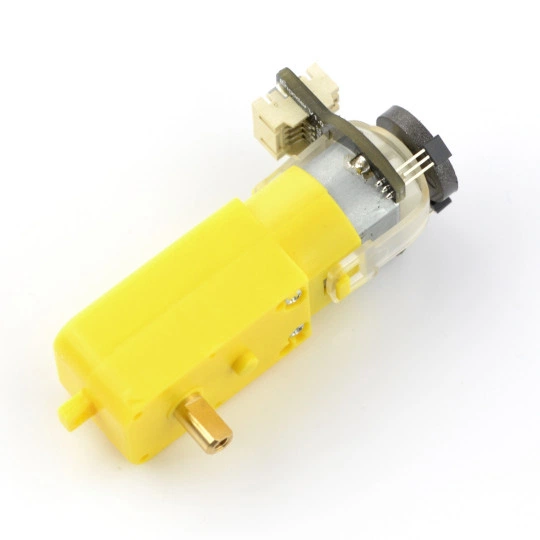
\includegraphics[width = 0.3\textwidth]{silnik_z_enkoder.png}
                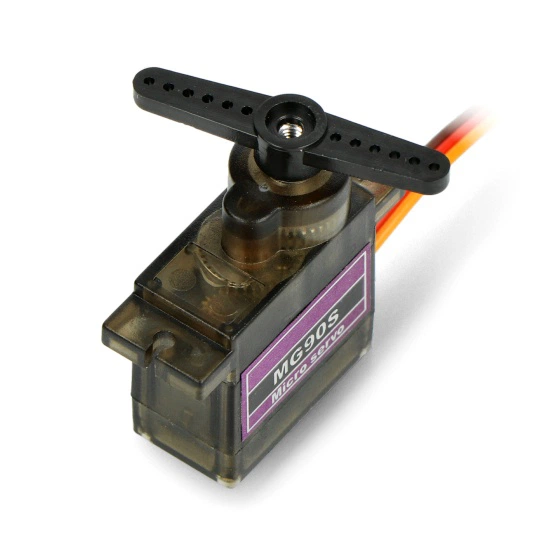
\includegraphics[width = 0.3\textwidth]{serwo_180.png}

                \caption{Silnik DC z enkoderem oraz serwomechanizmy $180^\circ$.}
                \footnotesize{Źródło: \href{https://botland.com.pl/}{botland.com}}
                % Źródło: https://botland.com.pl/silniki-dc-z-przekladnia-i-enkoderami/6287-silnik-z-przekladnia-sj01-120-1-6v-160rpm-enkoder-6959420910205.html
                % Źródło: https://botland.com.pl/serwa-typu-micro/20435-serwo-mg-90s-micro-180-stopni-metalowa-przekladnia-5904422380915.html
                \label{fig:engines}
            \end{figure}

        \subsubsection{Pomiar odległości}
            Autonomia pojazdu, nie ogranicza się wyłącznie do sterowania silnikami.
            Pojazd tego typu musi być świadomy swojego otoczenia, a do tego najlepiej sprawdzają się czujniki pozwalające na pomiar odległości.
            Poniżej przedstawiono listę kilku czujników:
            \begin{enumerate}
                \item Czujnik ultradźwiękowy -- najtańsze układy do pomiaru odległości, bardzo prymitywne.
                O bardzo niestabilnym pomiarze. Dodatkową zaletą jest prostota działania, jednak olbrzymią wadą czas wymagany do wykonania pomiarów.
                \item Czujniki Time of Flight (ToF) -- złożone wyspecjalizowane moduły pozwalające na dużą dokładność pomiarową oraz bardzo daleki zasięg.
                Zazwyczaj wymagają specjalnych bibliotek dostarczonych przez producenta - co stanowi zarówno wadę jak i zaletę. Takie czujniki mogą być bardzo szybkie, jednak złożona uniwersalna biblioteka, znacząco spowalnia pracę.
                \item Układy obiciowe IR -- proste dwu diodowe układy emitera i pomiaru natężenie światła podczerwonego. Układy o małej dokładności pomiarowej, dużej strefie martwej, niewielkim zakresie pomiarowym (od $2cm$ do $20cm$), małej stabilności pomiarowej -- pomiar zależy od koloru obiektu.
                \item Lidar -- wyspecjalizowane układy, pozwalające na bardzo precyzyjny pomiar w pełnym zakresie $360^\circ$ w okół pojazdu.
                Jedna z najlepszych dostępnych i przedstawionych opcji, jednak ceny takich układów, są zaporowe.
                \item Radar -- bardzo drogie i bardzo dokładne układy pomiarowe, pozwalające na niezwykła precyzję. Niestety, praktycznie nie dostępne w względnie małych rozmiarach na rynku konsumenckim. Dodatkowo wymają specjalnych procesorów sygnałowych pozwalających w miarę na bieżąco przetwarzać dane z radarów.
            \end{enumerate}
            Z przedstawionej listy, najlepszymi układami do tego zastosowania, wydają się czujniki typu ToF.
            Dodatkowo, w celach bezpieczeństwa z tyłu pojazdu zostały zamontowane czujniki IR, ale nie jako urządzenia pomiarowe, pozwalające zmierzyć odległość do przeszkody.
            Tylko jako czujniki zbliżeniowe, umożliwiające wykrycie przeszkody i zahamowanie przed zderzeniem.

    \subsection{Środowisko programistyczne}
        Następnym bardzo ważnym wyborem jest środowisko programistyczne, w którym zostanie zbudowany projekt.
        Tutaj też w ostatnich latach użytkownicy dostali olbrzymie możliwość wyboru.
        Podstawowymi rozwiązaniami dla programistów embedded są:
        \begin{enumerate}
            \item Eclipse -- kiedyś bardzo popularny, posiadający olbrzymi zbiór dodatków.
            Jest także rozprowadzany na otwartej licencji dlatego stanowi świetną bazę dla wielu bardziej zaawansowanych projektów.
            \item STM32 Cube -- środowisko przeznaczone strike do pracy z modułami STM32, oparte na Eclipsie.
            \item Atmel Studio -- środowisko przeznaczone do pracy z mikrokontrolerami z rodziny AVR od firmy ATmel.
            \item Keil µVision -- środowisko ogólnego przeznaczenia do pracy z układami Cortex, ograniczone licencją.
            \item Notepad++ -- bardziej zaawansowany notatnik, pozwalający na auto uzupełnianie słów. Na też masę wtyczek, pozwalających na stworzenie z niego pełnoprawnego środowiska programistycznego, jednak w swojej pierwotnej wersji bardzo trudny w użyciu.
            \item VS Code -- bardzo uniwersalne narzędzie, mające olbrzymią masę dodatków, pozwalających przystosować środowisko w pełni pod własne wymagania.
            Samo środowisko jest zbudowane na silniku przeglądarki internetowej, dzięki czemu może z powodzeniem zastąpić przeglądarkę PDF, a w wbudowany tile menedżer pozwala układać całość w bardzo czytelny sposób.
        \end{enumerate}
        Projekt został, zbudowany w środowisku VS Code, ze względu na największą elastyczność oraz możliwość dostosowania go do własnych potrzeb.


    \subsection{Środowisko CAD}
        Zbudowanie pojazdu autonomicznego wymaga wymodelowania odpowiednich części.
        % Dodatkowo, praca wymagała zaprojektowania kilku dodatkowych elementów mechanicznych.
        W tym celu, zostało wykorzystane środowisko CAD, które pozwala na zbudowanie modelu 3D.
        Poniżej przedstawiono listę kilku najpopularniejszych programów do projektowania.
        \begin{enumerate}
            \item SolidWorks -- program stworzony przez firmę Dassault Systemes, który jest bardzo popularny w przemyśle. Jest też niezwykle precyzyjny i każda operacja wymaga zastanowienia się dokładnie co chce się osiągnąć - przez co próg wejścia jest bardzo wysoki.
            \item Fusion 360 -- program stworzony przez firmę Autodesk, przeznaczony specjalnie do modelowania 3D. Posiada olbrzymie wsparcie dla drukarek 3D, a także dla obrabiarek CNC.
                                Jest także niezwykle intuicyjny a próg wejścia jest bardzo niski. Jedyną wadą programu, jest możliwość jedynie pracy w chmurze.
            \item FreeCAD -- darmowy program do projektowania modeli 3D, bardzo prosty w obsłudze, a nauczenie się tego programu wymaga naprawdę niewielkiego wkładu pracy.
                             Program jest stale rozwijany, a społeczność wokół niego ma możliwość rozbudowywania go o nowe funkcje. Niewątpliwą zaletą w porównaniu do innych programów jest możliwość uruchomienia go na każdym systemie operacyjnym.
        \end{enumerate}

        W projekcie został wykorzystany program FreeCAD, ze względu na swoją prostotę oraz możliwość uruchomienia na systemie Linux.

